

\section{Prueba 5}

\subsection{Red de inferencia}
\begin{center}
	\tikzstyle{regla}= [rectangle,draw,black,fill=blue!15]
	\tikzstyle{hecho}= [rectangle,draw,black,fill=black!15]
	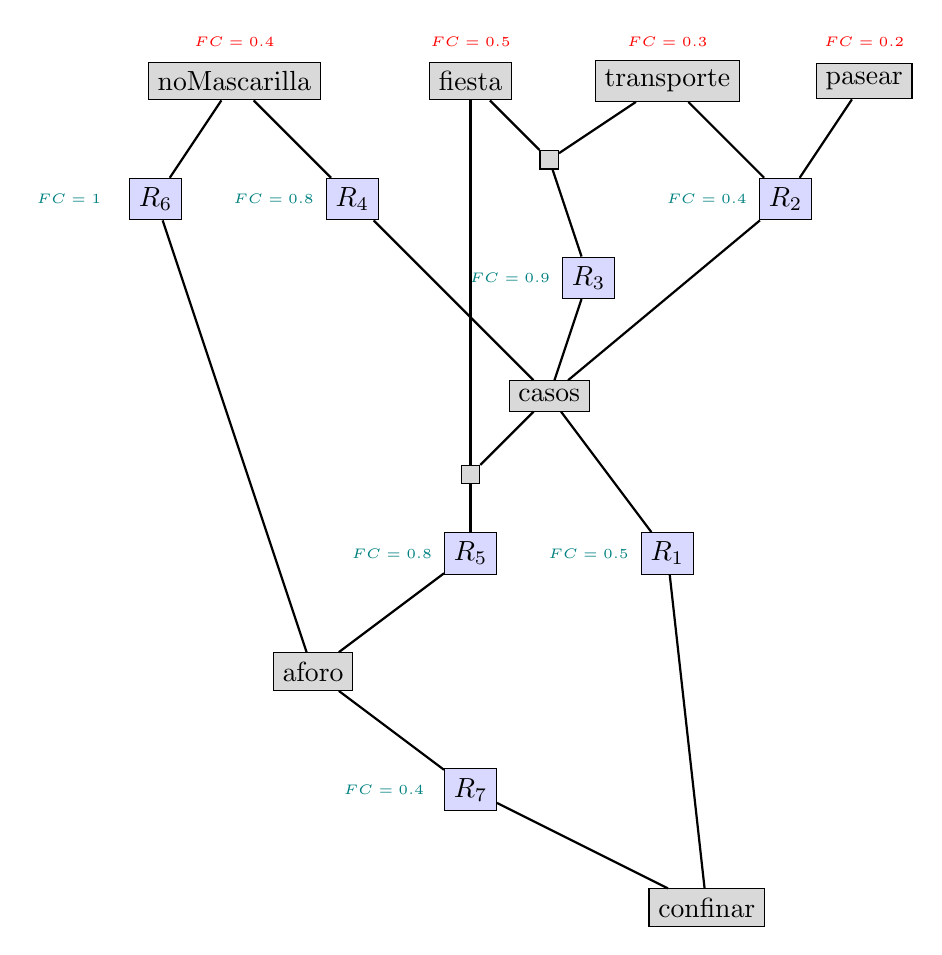
\begin{tikzpicture}
		
		\node (a) at (-4,5) [hecho] {noMascarilla};
		\node at (-4,5.5) {\color{red}{\tiny{$FC=0.4$}}};

		\node (b) at (-1,5) [hecho] {fiesta};
        \node at (-1,5.5) {\color{red}{\tiny{$FC=0.5$}}};

		\node (c) at (1.5,5) [hecho] {transporte};
		\node at (1.5,5.5) {\color{red}{\tiny{$FC=0.3$}}};

		\node (d) at (4,5)[hecho] {pasear};
        \node at (4,5.5) {\color{red}{\tiny{$FC=0.2$}}};

		\node (e) at (0,1)[hecho] {casos};
		
		\node (f) at (-3,-2.5)[hecho] {aforo};

        \node (g) at (2,-5.5)[hecho] {confinar};

		\node (b/c) at (0,4)[hecho] {};
        \node (b/e) at (-1,0)[hecho] {};

		\node (r1) at (1.5,-1) [regla] {$R_{1}$};
		\node at (0.5,-1) {\color{teal}{\tiny{$FC=0.5$}}};
		\node (r2) at (3,3.5) [regla] {$R_{2}$};
		\node at (2,3.5) {\color{teal}{\tiny{$FC=0.4$}}};
		\node (r3) at (0.5,2.5) [regla] {$R_{3}$};
		\node at (-0.5, 2.5) {\color{teal}{\tiny{$FC=0.9$}}};
		\node (r4) at (-2.5,3.5) [regla] {$R_{4}$};
		\node at (-3.5,3.5) {\color{teal}{\tiny{$FC=0.8$}}};
		\node (r5) at (-1,-1) [regla] {$R_{5}$};
		\node at (-2,-1) {\color{teal}{\tiny{$FC=0.8$}}};
		\node (r6) at (-5,3.5) [regla] {$R_{6}$};
		\node at (-6.1,3.5) {\color{teal}{\tiny{$FC=1$}}};
        \node (r7) at (-1,-4) [regla] {$R_{7}$};
		\node at (-2.1,-4) {\color{teal}{\tiny{$FC=0.4$}}};
		
		\path[black,thick] (a) edge[] node {} (r4);
        \path[black,thick] (r4) edge[] node {} (e);
        \path[black,thick] (e) edge[] node {} (b/e);
        \path[black,thick] (b/e) edge[] node {} (r5);
        \path[black,thick] (r5) edge[] node {} (f);
        \path[black,thick] (r6) edge[] node {} (f);
        \path[black,thick] (f) edge[] node {} (r7);

        \path[black,thick] (e) edge[] node {} (r1);
        \path[black,thick] (r1) edge[] node {} (g);
        \path[black,thick] (g) edge[] node {} (r7);
        \path[black,thick] (a) edge[] node {} (r6);

        \path[black,thick] (b) edge[] node {} (b/e);
        \path[black,thick] (b) edge[] node {} (b/c);
        \path[black,thick] (c) edge[] node {} (b/c);
        \path[black,thick] (b/c) edge[] node {} (r3);
        \path[black,thick] (r3) edge[] node {} (e);

        \path[black,thick] (c) edge[] node {} (r2);
        \path[black,thick] (d) edge[] node {} (r2);
        \path[black,thick] (r2) edge[] node {} (e);


	\end{tikzpicture}
\end{center}
\par Esta red de inferencia se debe interpretar de arriba a abajo.
Los rectángulos azules son las reglas, los grises que están ligados por encima 
de ellas son sus antecedentes, si estos antecedentes convergen en un cuadrado 
quiere decir que es la conjunción de esos literales, en caso contrario son disyunciones
o simplemente un literal. Los rectángulos grises que cuelgan de las reglas 
son sus consecuentes respectivamente. Además, incluyo los factores de certeza propocionados por
la Base de hechos y la Base de Conocimiento iniciales.
\subsection{Proceso de inferencia}

\subsection{Objetivo obtenido por SBR-FC}

